\documentclass[nopacs,nokeys]{revtex4}
\usepackage{amsmath}
\usepackage{amssymb}
\usepackage[utf8]{inputenc}
\usepackage{tcolorbox}
\usepackage{color}
\usepackage{tikz}
\usetikzlibrary{trees}
\usetikzlibrary{snakes}
\usetikzlibrary{positioning,decorations.pathmorphing}
\usetikzlibrary{decorations.markings}
\usepackage{tikz,ifthen}
\tikzset{beamerprimary/.style={structure.fg, thick}}
\tikzset{beamersecondary/.style={structure.bg, thick}}
\tikzset{ boson/.style={decorate, decoration={snake}},
     gauge/.style={decorate,decoration={snake,post length=1mm}}  ,
     fermion/.style={postaction={decorate},decoration={markings,mark=at position .55 with {\arrow{>}}}},
    fermionloop/.style={postaction={decorate},
        decoration={markings,mark=at position .25 with {\arrow{<}}}}, 
    gluon/.style={decorate, 
        decoration={coil,amplitude=4pt, segment length=5pt}},
    scalar/.style={dotted,postaction={decorate},decoration={markings,mark=at position .75 with {\arrow{>}}}},
    graviton/.style={double},
    dm/.style={double,postaction={decorate},decoration={markings,mark=at position .55 with {\arrow{>}}}},
}

\begin{document}

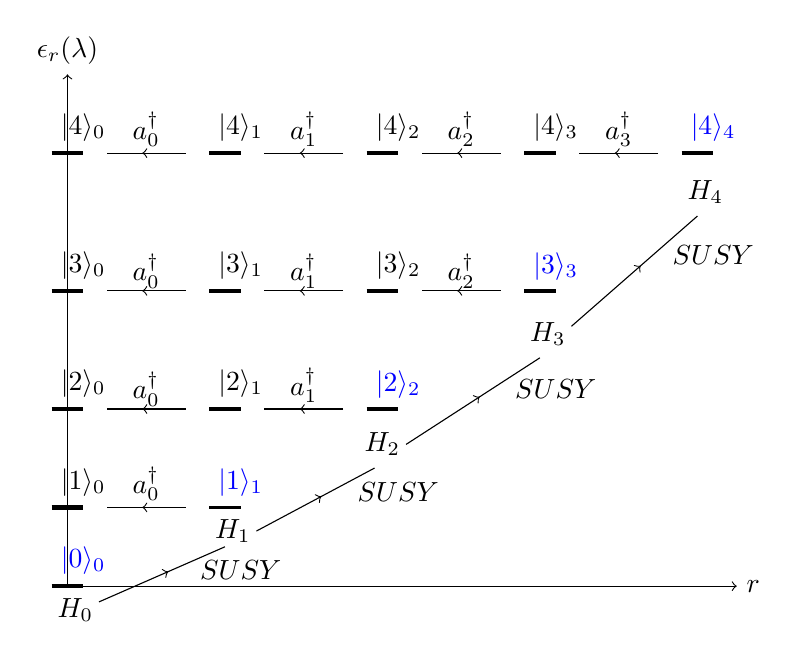
\begin{tikzpicture}
\draw[black,->] (0, 0)--(0,6.5) node[above]{$\epsilon_{r}(\lambda)$} ;
\draw[black,->] (0, 0)--(8.5,0)  node[right]{$r$} ;
%
\draw[black,ultra thick] (-0.2,0)--(0.2,0)  node[above ]{{\color{blue}$|0\rangle_{0}$}} ; 
\draw(0.1,-0.3)node{$H_{0}$};
\draw[black,ultra thick] (-0.2,1)--(0.2,1)  node[above ]{$|1\rangle_{0}$} ; 
\draw[black,ultra thick] (-0.2,2.25)--(0.2,2.25)  node[above ]{$|2\rangle_{0}$} ; 
\draw[black,ultra thick] (-0.2,3.75)--(0.2,3.75)  node[above ]{$|3\rangle_{0}$} ; 
\draw[black,ultra thick] (-0.2,5.5)--(0.2,5.5)  node[above ]{$|4\rangle_{0}$} ; 
%
\draw[fermion] (0.4,-0.2)-- (2,0.5);
\draw(2.2,0.2) node {$SUSY$} ;
\draw[fermion] (1.5,1)-- (0.5,1) ;
\draw(1,1.3) node {$a^{\dagger}_{0}$};
\draw[fermion] (1.5,2.25)-- (0.5,2.25) ;
\draw(1,2.5) node {$a^{\dagger}_{0}$};
\draw[fermion] (1.5,3.75)-- (0.5,3.75) ;
\draw(1,4) node {$a^{\dagger}_{0}$};
\draw[fermion] (1.5,5.5)-- (0.5,5.5) ;
\draw(1,5.8) node {$a^{\dagger}_{0}$};
%
\draw[black,very thick] (1.8,1)--(2.2,1)  node[above ]{{\color{blue}$|1\rangle_{1}$}} ; 
\draw(2.1,0.7)node{$H_{1}$};
\draw[black,ultra thick] (1.8,2.25)--(2.2,2.25)  node[above ]{$|2\rangle_{1}$} ; 
\draw[black,ultra thick] (1.8,3.75)--(2.2,3.75)  node[above ]{$|3\rangle_{1}$} ; 
\draw[black,ultra thick] (1.8,5.5)--(2.2,5.5)  node[above ]{$|4\rangle_{1}$} ; 
%
\draw[fermion] (2.4,0.7)-- (3.9,1.5);
\draw(4.2,1.2)node {$SUSY$} ;
\draw[fermion] (3.5,2.25)-- (2.5,2.25) ;
\draw(3,2.55) node {$a^{\dagger}_{1}$};
\draw[fermion] (3.5,3.75)-- (2.5,3.75) ;
\draw(3,4) node {$a^{\dagger}_{1}$};
\draw[fermion] (3.5,5.5)-- (2.5,5.5) ;
\draw(3,5.8) node {$a^{\dagger}_{1}$};
%
\draw[black,very thick] (3.8,2.25)--(4.2,2.25)  node[above ]{{\color{blue}$|2\rangle_{2}$}} ; 
\draw(4,1.8)node{$H_{2}$};
\draw[black,ultra thick] (3.8,3.75)--(4.2,3.75)  node[above ]{$|3\rangle_{2}$} ; 
\draw[black,ultra thick] (3.8,5.5)--(4.2,5.5)  node[above ]{$|4\rangle_{2}$} ; 
%
\draw[fermion] (4.3,1.8)-- (6,2.9);
\draw(6.2,2.5)node {$SUSY$} ;
\draw[fermion] (5.5,3.75)-- (4.5,3.75) ;
\draw(5,4) node {$a^{\dagger}_{2}$};
\draw[fermion] (5.5,5.5)-- (4.5,5.5) ;
\draw(5,5.8) node {$a^{\dagger}_{2}$};
%
\draw[black,very thick] (5.8,3.75)--(6.2,3.75)  node[above ]{{\color{blue}$|3\rangle_{3}$}} ; 
\draw(6.1,3.2)node{$H_{3}$};
\draw[black,ultra thick] (5.8,5.5)--(6.2,5.5)  node[above ]{$|4\rangle_{3}$} ; 
%
\draw[fermion] (6.4,3.3)-- (8,4.7);
\draw(8.2,4.2)node {$SUSY$} ;
\draw[fermion] (7.5,5.5)-- (6.5,5.5) ;
\draw(7,5.8) node {$a^{\dagger}_{3}$};
%
\draw[black,ultra thick] (7.8,5.5)--(8.2,5.5)  node[above ]{{\color{blue}$|4\rangle_{4}$}} ; 
\draw(8.1,5)node{$H_{4}$};
%
\end{tikzpicture}

\end{document}